\section{Maximal planar graphs}
This section will demonstrate a postprocessing approach for an already given straight-line drawing of a maximal planar graph $G$, namely $\Gamma_G$, in order to minimize the edge-length ratio of planar graphs.\\
The main idea is to elongate the shortest edge as long as possible while still maintaining planarity. Obviously, the longest edge of $\Gamma_G$ will not be altered at all. The small length edges may be enclosed by small area faces which proves to be a challenge for a required elongation. In order to overcome this hurdle, the grid will be refined as much as is necessary. On the one hand, this increases the total area usage of the new drawing $\Gamma'_G$, but will provide sufficient area for any small length edge elongation on the other hand.\\
After the grid refinement, every inner face of $G$ will be subdivided evenly. For every face, a new vertex will be inserted which is adjacent to the vertices defining the face. This will extend $G$ to the supergraph $G'$. In the further process, the inserted edges and vertices serve as a guideline for the edge elongations.\\
Then, every straight line edge of $G$ that is smaller than the longest edge will be elongated using a linear amount of bends, altering the straight-line drawing to a poly-line drawing. The line segments will stay in the respective adjacent faces defined by $G'$. The reader will observe that the amount of bends and the factor of grid refinement will play along and the edge-length ratio will become a constant.


% Initial situation

\subsection{Initial situation}
At the beginning, a given straight-line drawing $\Gamma_G$ of a planar graph $G$ is given. We choose the drawing algorithm by Schnyder. The area consumption values $(n-1)\times(n-1)$ in the worst case \cite{Schnyder}.
When considering maximal planar graphs, the following fact describes the shape of every face of $G$.
\begin{fact}\label{fact:maximal-triangle}
\end{fact}
In a maximal planar graph $G$, every face is a triangle. Otherwise, $G$ is not maximal planar.
\begin{proof}[Proof by contradiction]
	Let $f$ be a face of $G$ defined by $k > 3$ vertices. Then, it is possible to insert at least one more edge into $f$, contradicting the maximal planarity of $G$.
\end{proof}

\bigskip
Regarding area consumption, the smallest possible face in $\Gamma_G$ is a triangle with two edges of \UL. If these smallest-area faces are adjacent to an edge, then there is no bend point on the grid availiable for further elongation. Each triangle consumes area of $\frac{1}{2}\UL^2$ and the length of $e$ cannot be increased.
\begin{figure}[H]
	\centering
	\begin{subfigure}{0.3\linewidth}
		\centering
		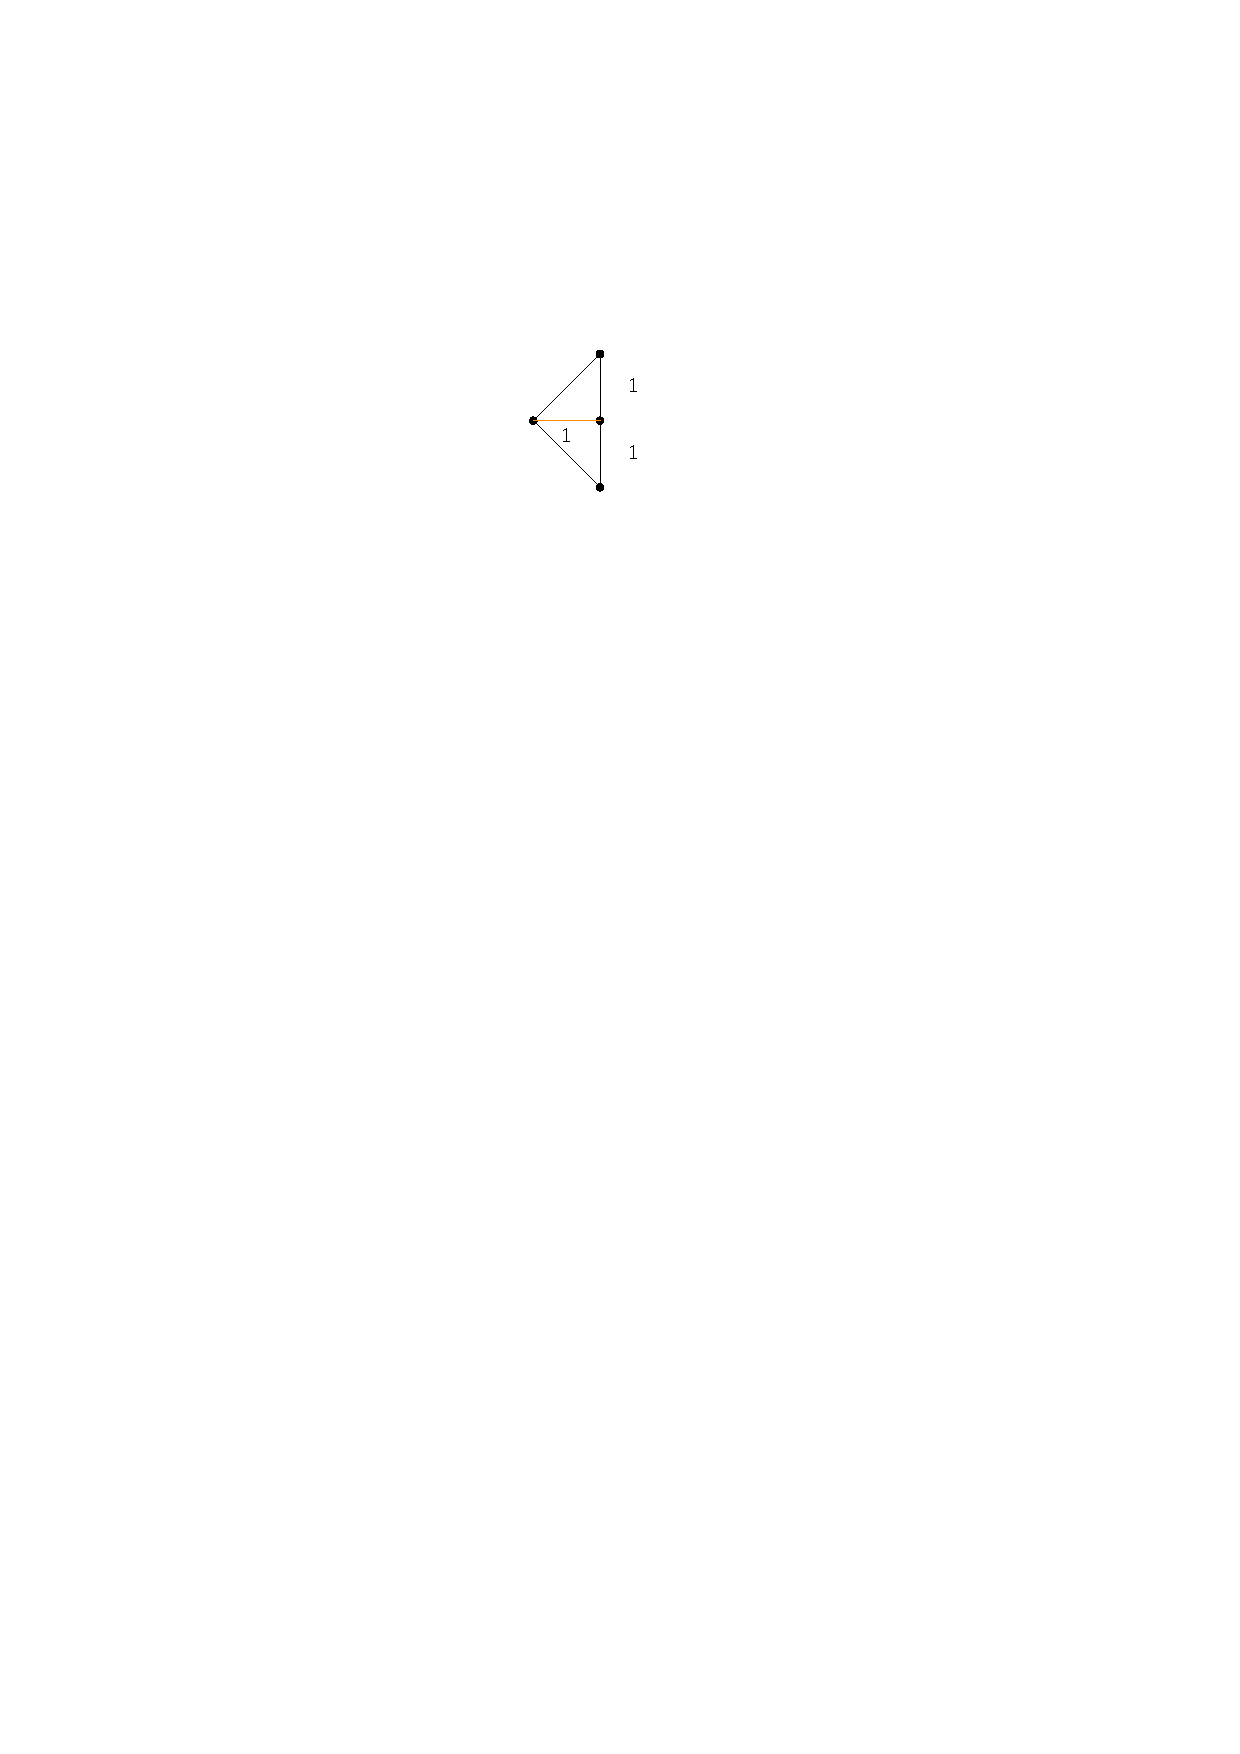
\includegraphics[width=0.7\textwidth,page=1]{drawings/maximal_planar.pdf}
	\end{subfigure}
\caption{An edge of \UL~(marked in orange), enclosed by two smallest-area triangles}\label{im:area_worst_case_straight-line}
\end{figure}
With a refinement in the first step, bend points are inserted into the adjacent triangles since their area consumption expands.


% Refinement

\subsection{Refinement step}
\begin{fact}\label{fact:area-expansion}
\end{fact}
Let $f$ be a face with an area consumption of $\mathcal{O}(a(k))$, $a(k)$ monotone increasing function and $k$ describing the granularity of the underlying grid. If the grid is refined by a factor of $c\cdot n$ for each dimension, then $f$ consumes area of $\mathcal{O}(c^2n^2 \cdot a(k))$.

\bigskip
So, by Fact \ref{fact:area-expansion}, the smallest possible area of a face now equals $\frac{1}{2}(cn)^2\UL^2$. Since every edge of unit length now is at least $c \cdot n$ long, the amount of bend points inside a face $f$ is bound by $\mathcal{O}((cn)^2)$. 
\begin{figure}[H]
	\centering
	\begin{subfigure}{0.3\linewidth}
		\centering
		\includegraphics[width=0.7\textwidth,page=2]{drawings/maximal_planar.pdf}
	\end{subfigure}
	\caption{The worst case from Figure \ref{im:area_worst_case_straight-line} after the refinement}\label{im:c-n_worst_case_straight-line}
\end{figure}
In the following sections, a straight-line drawing $\Gamma_G$ refined by a certain factor will be called $\Gamma'_G$, since the coordinates of the vertices changed. Although the shapes of the faces will stay the same, the area consumption is a different one.

% Supergraph extension

\subsection{Extending $G$ to a supergraph $G'$}
The supergraph is helpful for any transition of straight-line edge to a poly-line edge. It will describe where valid bend points lie. At first, the properties of maximal planar graphs is 

\begin{fact}\label{fact:even-subdivision}
\end{fact}
Let $f$ be a face of a drawing $\Gamma'_G$ with a constant amount of vertices defining it, inheriting area $\Theta(f(n))$. If $G$ is extended in a way that a new vertex, connected to all the vertices defining $f$, is placed inside $f$ so that $f$ is divided evenly, the resulting faces of the supergraph have still area $\Theta(f(n))$.
\begin{proof}
	Let $a$ be the area consumption of a face $f$, $a \in \Theta(f(n))$. Since the face is divided evenly by a constant amount $c$, every new face consumes at most $\frac{a}{c}+\varepsilon$ area and at least $\frac{a}{c}+\varepsilon'$ area $(\varepsilon,\varepsilon'>0)$. $\varepsilon, \varepsilon'$ describe the rounding error derived from the grid.
	\begin{align*}
		a \in \Theta(f(n)) \Rightarrow \frac{a}{c}+\varepsilon, \frac{a}{c}-\varepsilon' \in \Theta(f(n))
	\end{align*}
\end{proof}

\bigskip
So, if the grid is refined by $c\cdot n$, then, the face inheriting area $\frac{1}{2}(cn)^2\UL^2$ can be subdivided into three faces of roughly area $\frac{1}{6}(cn)^2\UL^2$ Since we are working on a grid with integers, there might be an approximation error which can be left out.

\begin{fact}\label{fact:maximal-planar-supergraph}
\end{fact}
Let $G$ be a maximal planar graph and $f$ a face of $G$. Extend $G$ to $G'$ by adding one vertex inside of $f$ and connecting to every vertex defining $f$. Then, $G'$ is maximal planar.
\begin{proof}
	If $f$ is an inner face, then it is a triangle with three vertices defining $f$. The vertex placed inside divides $f$ into three triangles, since it is connected to every of the three vertices defining $f$. $G'$ has now $v+1$ vertices, three more edges and one face is substituted with three smaller faces. Therefore, the amount of faces is increased by two and Eulers Formula holds.\\
	If $f$ is the outerface, then there are three vertices on the outerface, as well. Otherwise, there would be edges addable to $G$, and $G$ is not planar. The same holds for this case. 
\end{proof}

\bigskip
The intendation behind the vertex insertions is to evenly subdivide every face into three distinct new faces so every edge adjacent to two faces will have its own area reserved to be elongated in. This ensures the planarity of the output poly-line drawing naturally. The next Fact will answer the question where for each face, the vertices are inserted in practice.	

\begin{fact}\label{fact:centroid-point}
\end{fact}
Let $A,B,C$ be three points on the grid with their respective x and y coordinates, defining a triangle. Then, there exists a point $M$, called the centroid, which divides the triangle into three smaller triangles with roughly the same area usage, apart from a rounding error \cite{Centroid}. This point is defined as the arithmetic mean of $A,B,C$:
$$M\left(\frac{1}{3}(A_x + B_x + C_x), \frac{1}{3}(A_y+B_y+C_y)\right)$$

\bigskip

After the refinement and the graph extension, there are now sufficient bend points in reserved areas for every edge of $G$ to be elongated in availiable.

% Elongation

\subsection{Elongation step}
The general goal is to level all edge lengths occurring in $\Gamma'_G$. It is a question of how many bends are used in practice. The more bends are availiable, the more line segments can be inserted inside of a face. In the following section, the factor of refinement is specified along with a lower bound of the worst case scenario - the unit length edge with the smallest-area triangles possible attached to it.
\begin{fact}[Valid bend points]
\end{fact}
A grid point $b$ regarding a face $f$ is \textit{valid} iff it lies inside $f$ and the minimal distance to an edge defining $f$ lies in $(0,1]$.
\begin{fact}[Zig-zag elongation]\label{fact:poly-line-area-length}
\end{fact}
Let $A$ be a bounding box with area consumption $\mathcal{O}(a(k))$, where $k$ describes a granularity of the underlying grid. The height and the width of $A$ is described as $\mathcal{O}(h(k)), \mathcal{O}(w(k))$, respectively.  \\
A poly-line $p$ can be drawn inside $A$ with length $\mathcal{O}(a(k))$, using $\mathcal{O}(\min\{ h(k),w(k) \})$ bends.
\begin{proof}
	Let w.l.o.g. the height be larger than the width. The other case is valid analogously. The valid bend points are placed at the top and bottom row along the width at the bounding box. Start at one left corner of $A$ and draw a line segment along the height. For the following line segments, alternate with bends points between the top and bottom row until a right corner of $A$ is reached. The amount of bends are at most two times the width length. The length of the poly-line $p$ is therefore at most:
	\begin{align*}
		len(p) \leq (2\cdot w(k)+2) \cdot h(k) \in \mathcal{O}(w(k)h(k))
	\end{align*}
\end{proof}

\begin{lemma}\label{lemma:minimum-length}
\end{lemma}
When the grid is refined by a factor of $c\cdot n$ in each dimension, every edge of $\Gamma'_G$ can be elongated up to a length of $\Omega((c\cdot n)^2)$, using $O(c\cdot n)$ bends.
\begin{proof}
	Consider an edge $e$ of $\Gamma_G$ with \UL, enclosed by two smallest-area triangle faces. After the refinement and graph extension to $\Gamma'_{G'}$, the area consumption of the faces adjacent to $e$ values $\mathcal{O}((cn)^2)$[Fact \ref{fact:even-subdivision} and \ref{fact:area-expansion}]. Using all valid bend points in both faces adjacent to $e$, $e$ can be redrawn with $c\cdot n - 5$ line segments.
	
	\begin{figure}[H]
		\centering
		\begin{subfigure}{0.3\linewidth}
			\centering
			\includegraphics[width=0.7\textwidth,page=3]{drawings/maximal_planar.pdf}
		\end{subfigure}
		\caption{Using all valid bend points for line segment insertions}\label{im:all_valid_bend_points}
	\end{figure}
	
	$e$ is redrawn with a zig-zag elongation, using $2\cdot (cn-5)$ valid bend points. The new length of the sequence of line segments values at least:
	\begin{align}
		len(e) &\geq 3\cdot \left(2\cdot \sum_{i=1}^{\frac{cn-1}{3}-1}i + \sum_{i=1}^{\frac{cn-1}{3}-1}\sqrt{4i^2+1}\right)\\
		&> 3\cdot \left(2\cdot \sum_{i=1}^{\frac{cn-1}{3}-1}i + 2 \sum_{i=1}^{\frac{cn-1}{3}-1}i\right)\\
		&= 12 \cdot \sum_{i=1}^{\frac{cn-1}{3}-1}i\\
		&= \frac{2}{3}(cn)^2-\frac{10}{3}cn-\frac{4}{3}~~~\in \mathcal{O}((cn)^2)\label{eq:minimum-length-cn}
	\end{align}
\end{proof}
\bigskip

With this minimum length of $e$, drawn with as many line segments as possible, the following result can be achieved.
\begin{theorem}
	Let $\Gamma_G$ be given. If the drawing is refined by the factor of $n^2$, then there is sufficient area in $\Gamma'_G$ to elongate every edge so that the edge-length ratio is a constant.
\end{theorem}
\begin{proof}
	By equation \ref{eq:minimum-length-cn}, using $\mathcal{O}(n^2)$ bends, any edge can be elongated up to a length of $\mathcal{O}(n^4)$ while the length of the longest straight-line edge in an area of $\mathcal{O}(n^3)\times\mathcal{O}(n^3)$ lies in $\mathcal{O}(n^3)$.
\end{proof}

\bigskip
In practice, the longest edge of a straight-line drawing will not be altered in the transition from $\Gamma_G$ to $\Gamma'_G$.\\
So, by a refinement of $n^2$, it might be possible lengthen the shortest edge so that it is longer than the longest edge of $\Gamma'_G$. When the shortest edge can get longer than the longest one, then the same applies for every edge. But, this requires up to $2n^2$ bends per edge and is a bit over the top. In the next section, we will determine, that a linear amount of bends suffice so that the ratio is a constant.
%% Summary
\subsection{Using $n$ bends}

In the last section, it was shown that a refinement by a factor of $n^2$ suffices to level the lengths of all edges. In this section, the number of bends used per edge is fixed to $n$. At first, it is shown that the edge-length ratio will still be a constant when using $n+1$ line segments in order to draw an edge. Secondly, with help of the worst case example, a lower bound for the edge lengths is determined. Finally, the ratio will be investigated.
\begin{lemma}
\end{lemma}
With a refinement by a factor of $n^2$ and using $n$ bends and the supergraph extension as described above, the edge length ratio of the resulting drawing will lie in $\mathcal{O}(1)$.
\begin{proof}
	With $n$ valid bends, $n+1$ line segments are inserted into reserved faces of at least $\mathcal{O}(n^2)\times \mathcal{O}(n^2)$ area. Since the bend points are valid ones, they lie at the boundary of the corresponding faces. When inserting a line segment on opposing bend points, its length will lie in $\mathcal{O}(n^2)$, since it spans over one dimension of the face. $n+1$ line segments of such sort sum up to a total length of $\mathcal{O}(n^3)$. The length of the longest straight-line edge in a $\mathcal{O}(n^3)\times\mathcal{O}(n^3)$ drawing is also in $\mathcal{O}(n^3)$, therefore the ratio lies in $\mathcal{O}(1)$.
\end{proof}

\bigskip
Next, a lower bound of edge length is determined for a specific kind of face of $G$ - a triangle consisting of a horizontal line segment with length $w$ - also the edge to be elongated - a vertical line segment of height $h$ and the enclosing diagonal line segment. 
\begin{figure}[H]
	\centering
	\begin{subfigure}{0.4\linewidth}
		\centering
		\includegraphics[width=0.9\textwidth,page=4]{drawings/maximal_planar.pdf}
		\caption{}
	\end{subfigure}
	\begin{subfigure}{0.4\linewidth}
		\centering
		\includegraphics[width=0.9\textwidth,page=5]{drawings/maximal_planar.pdf}
		\caption{}
	\end{subfigure}
	\caption{A general width $w$ and height $h$, before (a) and after (b) grid refinement and graph extension}\label{im:h_greater_3w}
\end{figure}
When recalling the position of the centroid [Fact \ref{fact:centroid-point}], there are two cases of line segment insertions:\\
\underline{Case 1:} $h > 3w$\\
In this case, the height of the face created by the supergraph extension is larger than the length of the edge of interest with length $w$. 
\begin{figure}[H]
	\centering
	\begin{subfigure}{0.4\linewidth}
		\centering
		\includegraphics[width=0.9\textwidth,page=6]{drawings/maximal_planar.pdf}
	\end{subfigure}
	\caption{Inserting vertical line segments}\label{im:vertical_insertion}
\end{figure}
The line segments of the new polyline are inserted vertically, using valid bend points so that all the inserted line segments are as long as possible. 

\underline{Case 2:} $h \leq 3w$\\
In this case, the length of the original edge $e$ will at least as long as the new height to the inserted centroid $M$ of $G'$. So, the line segments will be placed horizontally, parallel to $e$. In order to preserve planarity, a bend point must be placed near the inserted vertex $M$. 
\begin{figure}[H]
	\centering
	\begin{subfigure}{0.4\linewidth}
		\centering
		\includegraphics[width=0.9\textwidth,page=7]{drawings/maximal_planar.pdf}
	\end{subfigure}
	\caption{Inserting horizontal line segments. The orange dotted bend points preserve planartiy}\label{im:horizontal_insertion}
\end{figure}
\begin{lemma}
\end{lemma}
For two positive integers $w,h>1$, it holds:
\begin{align*}
	\frac{hn^2-1}{wn^2-1}<h
\end{align*}
\begin{proof} The two cases of line segment insertions are covered with the following two cases:
	\begin{itemize}
		\item \underline{Case 1:} $h>w$\\
		\begin{align*}
			\frac{hn^2-1}{wn^2-1} < \frac{hn^2-n^2}{wn^2-n^2} = \frac{h-1}{w-1}< h
		\end{align*}
		\item \underline{Case 2:} $h \leq w$\\
		\begin{align*}
			\frac{hn^2-1}{wn^2-1} \leq \frac{hn^2}{wn^2} = \frac{h}{w} < h
		\end{align*}
	\end{itemize}
\end{proof}
\begin{lemma}
	When inserting up to $\frac{n}{2}$ line segments horizontally or vertically, depending on the height and the width of the face, the length of the resulting poly-line equals at least $n^3 - \mathcal{O}(n^2)$.
\end{lemma}

\begin{proof}
	\begin{itemize}
		\item Case 1: $h > 3w$\\		
		Let $f$ be a face in $\Gamma'_G$ defined by an horizontal edge $e = \overline{AB}$ with length $w' = w\cdot n^2$, w.l.o.g. a vertical line segment $\overline{BC}$ of length $h'=h\cdot n^2$, and the enclosing diagonal line segment. When the graph is extended to $G'$, the centroid is placed in $\Gamma'_{G'}$ at:
		\begin{align*}
			M\left(\frac{1}{3}(A_x+B_x+C_x) , \frac{1}{3}(A_y+B_y+C_y) \right)
		\end{align*}
		Since the x-coordinate of $B$ equals the one from $C$ and the y-coordinate of $A$ equals the one of $B$, it holds:
		\begin{align*}
			M\left(\frac{1}{3}A_x+\frac{2}{3}B_x , \frac{1}{3}C_y+\frac{2}{3}A_y \right)
		\end{align*}
		For further length calculations, the point $A$ is placed on the origin of the coordinate system. Then, the points are defined as follows:
		\begin{align*}
			A&(0,0)\\
			B&(w'-1,0)\\
			C&(w'-1,h'-1)\\
			M&\left(\frac{2}{3}(w'-1),\frac{1}{3}(h'-1)\right)
		\end{align*}
		\begin{figure}[H]
			\centering
			\begin{subfigure}{0.8\linewidth}
				\centering
				\includegraphics[width=0.9\textwidth,page=10]{drawings/maximal_planar.pdf}
			\end{subfigure}
			\caption{When $A$ is placed on the origin, this figure shows the positions and linear function descriptions of the faces}\label{im:coordinate_properties}
		\end{figure}
	
		When the y-coordinate of $M$ is greater than $w'$, then vertically inserted line segments will be longer than horizontally inserted ones. The elongation with $n$ bends and $\frac{n}{2}$ vertical line segments looks as follows:
		\begin{figure}[H]
			\centering
			\begin{subfigure}{0.6\linewidth}
				\centering
				\includegraphics[width=0.9\textwidth,page=8]{drawings/maximal_planar.pdf}
			\end{subfigure}
			\caption{Inserting vertical line segments in one face only}\label{im:vertical_one_face}
		\end{figure}
		And the lower bound of the total length can be estimated by the sum of the length of vertical line segments times two, since the diagonal line segments are at least as long as the vertical ones.
		\begin{align}
			len(e') &\geq \frac{1}{3}hn^2\cdot \frac{n}{2}-\left(1+\frac{1}{2}\left(\frac{h'-1}{w'-1}\right)\sum_{i=1}^{\left(\frac{n}{2}-1\right)\cdot\frac{2}{3}}i\right)-\left(\frac{h'-1}{w'-1}\sum_{i=1}^{\left(\frac{n}{2}-1\right)\cdot\frac{1}{3}}i\right)\label{eq:vertical}\\
			&+ \frac{1}{3}hn^2\left(\frac{n}{2}-1\right)-\frac{1}{2}h\frac{\left(\frac{n}{3}-\frac{2}{3}\right)\left(\frac{n}{3}+\frac{1}{3} \right)}{2}-h\frac{\left(\frac{n}{6}-\frac{1}{3}\right)\left(\frac{n}{6}+\frac{2}{3}\right)}{2}\label{eq:vertical-connectors}\\
			&=\frac{1}{3}hn^3-\left(\frac{4}{9}h-\frac{1}{2}w\right)n^2+\frac{1}{3}h
		\end{align}
	Since $h>3w$ and $h,w\geq1$, the length of the poly-line values at least $wn^3-\mathcal{O}(n^2)$ and the statement holds.
		\item Case 2: $h \leq 3w$
	In this case, the original straight line will be substituted with one horizontal line segment starting at $A$, ending in a bend point right before $B$. Furthermore, there will be a bend point right below $C$ in order to preserve planarity. The other horizontal line segments will be placed above the bottom one between $A$ and $B$. The line segments are shortened by $w$ from the right side and $2w$ from the left side, in total $3w$ per insertion. Since we only consider one face, the number of bend points and line segments is halved. 
	\begin{figure}[H]
		\centering
		\begin{subfigure}{0.6\linewidth}
			\centering
			\includegraphics[width=0.9\textwidth,page=9]{drawings/maximal_planar.pdf}
		\end{subfigure}
		\caption{Inserting $\frac{n}{4}$ horizontal line segments. The orange dotted bend point preserves planartiy}\label{im:horizontal_one_face}
	\end{figure}
	Then, the following lower bound for the length can be calculated:
	\begin{align}
		len(e') &\geq wn^2\cdot\left(\frac{n-2}{4}-3w\sum_{i = 1}^{\frac{n-2}{4}}i\right)\label{eq:horizontals}\\
		&+ wn^2\cdot \left(\frac{n-2}{4}-1\right)-3w\sum_{i=1}^{\frac{n-2}{4}-1}i\\
		&= \frac{1}{2}wn^3-\frac{35}{16}wn^2+\frac{3}{4}wn-\frac{3}{16}w
	\end{align}		
	This length is achieved by using the area of one adjacent face to $e$. However, this length is doubled when using both adjacent faces. The total length then values at least $wn^3-\mathcal{O}(n^2)$ and since  $w,h\geq1$, the statement holds.
	\end{itemize}
\end{proof}

\bigskip
\begin{lemma}
	The calculated minimum length also holds for any edge of $G$, regardless of the orientation of the adjacent faces.
\end{lemma}
\begin{proof}
	Since every face is a triangle, the defining line segments can always be described with help of a linear function $f(x)=mx+b$, as already done in Figure \ref{im:coordinate_properties}. Consider a valid bend point $K$. Then, the next valid point lies either above or below by one row, or left or right by one column. The actual position is determined by the slope of the linear function, describing the line segment next to $K$. This slope is a constant. So, by inserting a new horizontal line segment above or below a preexisting one occupying $K$, or by inserting a new vertical line segment left or right a preexisting one occupying $K$, the difference of length between those inserted line segments is a constant one. Therefore, the resulting length of the zig-zag line is of form $n^3-\mathcal{O}(n^2)$.
\end{proof}
\begin{theorem}\label{theorem:minimum-polyline-length}
\end{theorem}
In $\Gamma'_{G'}$, every edge of $G$ can be elongated to a poly-line with a length of at least $n^3 - \mathcal{O}(n^2)$, using $n$ bends.
\begin{proof}
	As a consequence of the refinement, every face $f$ inherits at least area of $\mathcal{O}(n^2)\times\mathcal{O}(n^2)$. When considering bend points only valid iff they lie on the boundary of $f$ and line segments must traverse the face, then there will be $n+1$ line segments inserted with a length of at least $n^2$, shortened by a linear amount in the worst case. This leads to $n$ line segments with length at least $n^2 - \mathcal{O}(n)$, summing up to a total length of at least $n^3-\mathcal{O}(n^2)$.
\end{proof}
\subsection{Summary}
The previous results can be summarized to the following theorems:
\begin{theorem}\label{theorem:max-planar-ratio1}
\end{theorem}
Let $G$ be a maximal planar graph, admitting a planar Schnyder straight-line grid drawing $\Gamma_G$ with a maximal area consumption of $(n-1)\times(n-1)$. Let $f(n)$ be a monotone function which describes the amount of bends per edge allowed. If $f(n) = n$, and the grid is refined by a factor of $n^2$, then $\Gamma_G$ can be altered to a poly-line drawing $\Omega_G$ such that the edge-length ratio lies in $\mathcal{O}(1)$ in area $\mathcal{O}(n^3) \times \mathcal{O}(n^3)$.
\begin{proof}
	Let $\Gamma_G$ be a Schnyder straight-line drawing of a maximal planar graph with $n$ vertices. Then, the edge-length ratio lies in $\mathcal{O}(n)$ since the length of the shortest edge values at least 1\UL~ and the length of the longest edge values at most $\sqrt{2}(n-1)$\\
	Refine the grid by a factor of $n^2$ in each dimension to obtain $\Gamma'_G$ in area $\mathcal{O}(n^3)\times \mathcal{O}(n^3)$. Then, by Fact \ref{fact:area-expansion}, every inner face consumes at least area of $\mathcal{O}(n^4)$.\\
	For each inner face $f$, a vertex is inserted and connected to each of the three vertices defining $f$. Mark the new vertices and edges. These new vertices extend $G$ to $G'$. $G'$ has $3n-6$ edges, there are 3 edges on the outerface and $3n-9$ inner edges. Every edge of $G$ is adjacent to two faces and enclosed by exactly four marked edges in $G'$. By Fact \ref{fact:even-subdivision}, the area enclosed by these marked edges is at least $\mathcal{O}(n^4)$ big and, by construction, this area is free in $\Gamma'_G$. By Fact \ref{fact:poly-line-length-equal-arbitrary-shape-area}, every edge of $G$ drawn in $\Gamma'_G$ can be elongated \grqq zig-zag wise\grqq~by a factor of $n$ bends used within the marked enclosing edges. For an edge of $G$ with length $\mathcal{O}(n^2)$ in $\Gamma_G'$, with $n$ bends the zig-zag elongation results in a length of $\mathcal{O}(n^3)$, by Theorem \ref{theorem:minimum-polyline-length} at least $n^3-\mathcal{O}(n^2)$ long. By leveling the length of all edges of $G$ to $\mathcal{O}(n^3)$ and deleting the edges and vertices of $G'\setminus G$ again, the result is a poly-line drawing $\Omega_G$ with an edge-length ratio of $\mathcal{O}(1)$ in area $n^2(n-1)\times n^2(n-1)$ and $n$ bends per edge.
\end{proof}
The following pseudocode sketches this drawing algorithm:\\
\begin{algorithm}[H]
	\KwIn{A Schnyder straight-line drawing $\Gamma_G$ in area up to $n-1\times n-1$}
	\KwOut{A poly-line drawing $\Omega_G$ with a minimized edge-length ratio}
	$\Gamma'_G \gets \Gamma_G.\texttt{RefineGrid}(n^2)$ \Comment{Grid refinement} \\
	$G'\gets G$\Comment{supergraph extension}\\
	\For{inner face $f$ of $G$}{
		$V(G') \gets V(G')\cup\{M_f\}$\Comment{$M_f$ subdivides $f$}\\
		$E(G') \gets E(G')\cup\{(M_f,A_f),(M_f,B_f),(M_f,C_f)\}$\Comment{$f$ defined by $A_f,B_f,C_f$}\\
		$\texttt{Pos}(M_f) = \frac{1}{3}\left(\texttt{Pos}(A_f)+\texttt{Pos}(B_f)+\texttt{Pos}(C_f)\right)$\\
		\texttt{DrawVertex}($M_f$)\\
		\texttt{MarkVertex}($M_f$)\\
		\texttt{DrawEdge}($\{(M_f,A_f),(M_f,B_f),(M_f,C_f)\}$)\\
		\texttt{MarkEdge}($\{(M_f,A_f),(M_f,B_f),(M_f,C_f)\}$)
	}

	$\texttt{float } l_{\max} \gets |\texttt{longestEdge}| $\\
	\For{edge $e$ in $E(G)$}{
		$\Gamma'_{G'}$\texttt{.EvalValidBendPoints($e$)}\Comment{Zig-zag elongation}\\
		\texttt{int bends}$\gets 0$\\
		\While{\texttt{bends}$<n-1 \wedge len(e)<l_{\max} $}{
			\texttt{bends}$\gets$\texttt{bends}$+2$\\
			\texttt{InsertLineSegment}$(e)$ \Comment{as long as possible}\\
			\texttt{DrawPolyLine}($e$)
		}
	}
	\For{$v \in V(G')$}{
		\If{$v$\texttt{.marked}}{$\Gamma'_{G'}$\texttt{.delete(v)}}
	}
	\For{$e \in E(G')$}{
	\If{$e$\texttt{.marked}}{$\Gamma'_{G'}$\texttt{.delete(e)}}
}
	\Return $\Gamma'_{G'}$	
	\caption{Modification of a straight-line drawing}
\end{algorithm}
\subsection{Runtime}
The above algorithm refines the grid by a factor of $n^2$, runtime $\mathcal{O}(n^2)$. Then, the subdivision takes place for every face, these are constant many operations for a linear amount of faces, ergo the runtime is $\mathcal{O}(n)$. The for loop in line 10 to 16: The validation of bend points may take $\mathcal{O}(n^3)$ since this is the area upper bound for the largest possible faces in a $\mathcal{O}(n^3)\times\mathcal{O}(n^3)$ drawing. And since there are a linear amount of edges (planar graph), the for loop may run in $\mathcal{O}(n^4)$ in the worst case. The deletion of the marked vertices and edges runs in linear time. The total runtime is therefore $\mathcal{O}(n^4)$.
\begin{theorem}
\end{theorem}
Every planar graph $G$ admits a poly-line drawing with an edge-length ratio of $\mathcal{O}(1)$ in area $\mathcal{O}(n^3)\times \mathcal{O}(n^3)$, allowing up to $n$ bends per edge.
\begin{proof}
	At first, add edges to $G$ so it is a maximal planar graph $G_{\max}$ and mark them. Then, draw $G_{\max}$ according to the proof of Theorem \ref{theorem:max-planar-ratio1}. The output is a poly-line grid drawing in area $\mathcal{O}(n^2)\times \mathcal{O}(n^2)$ with an edge-length ratio of $\mathcal{O}(1)$ and up to $\mathcal{O}(n)$ bends per edge. Afterwards, remove all marked edges from $G_{\max}$ to obtain $\Omega_G$.
\end{proof}

The following observation describes the behaviour of the ratio of large-scale graphs.
\begin{observation}
\end{observation}
Assuming, the base straight-line drawing $\Gamma_G$ is a Schnyder drawing, then with a refinement of $n^2$ and a usage of $n$ bends the edge-length ratio converges to $\sqrt{2}$ for $n \to \infty$.
\begin{proof}
	In a Schnyder straight-line drawing $\Gamma_G$, the area consumed values $n-1\times n-1$. The length of the longest edge values at most $\sqrt{2}(n-1) < \sqrt{2}n$. After the refinement by a factor of $n^2$, the longest edge values at most $\sqrt{2}n^3$. The ratio $r_G$ can then be expressed as:
	\begin{align*}
		r_G = \frac{\sqrt{2}n^3}{n^3-\mathcal{O}(n^2)} \underbrace{\rightarrow}_{n\to\infty} \sqrt{2}
	\end{align*}
\end{proof}
It is intuitive that for large scale graphs, the ratio might be better than for small-scale graphs. A refinement by a larger factor enables more bend points and alternations, leading to a better approximation for the edge-length levelling.
\begin{observation}
\end{observation}
Let $\Omega_G$ be a poly-line drawing of $G$ with a ratio of $r$, using $n$ bends. When the number ob bends is increased to $r\cdot n$, then the ratio tends to 1 for large-scale graphs.

\bigskip
The reason for this to happen is that every line-segment of the polyline has length at least $n^2 - \mathcal{O}(n)$. Using $r$ poly-lines, the length would be of form $r\cdot n^3 - \mathcal{O}(n^2)$. For large scale graphs, this might tend to 1. 

\subsection{An Example}\label{section:max_planar_example}
In order to see the whole postprocessing, the ratio of a straight-line drawing of the complete graph $K_4$ is minimized. The input is a straight-line drawing $\Gamma_{K_4}$ on a grid of size $3\times3$.
	\begin{figure}[H]
	\centering
	\begin{subfigure}{0.6\linewidth}
		\centering
		\includegraphics[width=0.9\textwidth,page=11]{drawings/maximal_planar.pdf}
	\end{subfigure}
	\caption{Input drawing of $K_4$ on a $3\times3$ grid}
\end{figure}
The ratio $r$ values $\sqrt{5}$, since the length of edge $(3,4)$ values 1 and the length of the edges $(1,4),(2,4)$ value $\sqrt{5}$.
Since $\mid V\mid = 4$, the grid is refined by $4\cdot 4$, resulting in a grid of size $48\times48$. The graph is extended, so that the area for edge elongations is defined.
	\begin{figure}[H]
	\centering
	\begin{subfigure}{0.6\linewidth}
		\centering
		\includegraphics[width=0.9\textwidth,page=12]{drawings/maximal_planar.pdf}
	\end{subfigure}
	\caption{Supergraph of $K_4$ on a $48\times48$ grid}
\end{figure}
Then, each edge is evaluated regarding its dashed cyan-colored bounding area and elongated with up to $n = 4$ bends.
	\begin{figure}[H]
	\centering
	\begin{subfigure}{0.6\linewidth}
		\centering
		\includegraphics[width=0.9\textwidth,page=13]{drawings/maximal_planar.pdf}
	\end{subfigure}
	\caption{Inserting up to 4 bends per edge for ratio minimization}
\end{figure}
	\begin{figure}[H]
	\centering
	\begin{subfigure}{0.6\linewidth}
		\centering
		\includegraphics[width=0.9\textwidth,page=14]{drawings/maximal_planar.pdf}
	\end{subfigure}
	\caption{$\Omega_{K_4}$}
\end{figure} 
For the edges $(1,2),(1,3),(2,3)$, the elongation was softened to approximate the longest edge. In order to demonstrate, what happens with maximum elongation, the previously shortest edge was elongated as long as possible. The calculated lengths are:
\begin{align}
	|(1,4)| = |(2,4)|&= 44,72\\
	|(1,2)| &= 44,39\\
	|(3,4)| &= 55,45\\
	|(1,3)| = |(2,3)| &= 43,56\\
	\Rightarrow r &= 1,28
\end{align}
The reason that $r$ is not quite optimal lies in the fact that the previously shortest edge became the longest edge. So, it seems that the algorithm requires further adjusting regarding the resulting edge lengths. The following alternative drawing inherits a nearly optimal ratio:
	\begin{figure}[H]
	\centering
	\begin{subfigure}{0.6\linewidth}
		\centering
		\includegraphics[width=0.9\textwidth,page=15]{drawings/maximal_planar.pdf}
	\end{subfigure}
	\caption{$\Omega'_{K_4}$}
\end{figure}
Here, $|(3,4)|=25,24$ and $r' = 1,04$. Nice.